\documentclass[10pt]{beamer}
\usepackage{../sty/open-cbgm-sbl-talk}
\title{The \texttt{open-cbgm} Library:\\Design and Demonstration}
\author{Joey McCollum\inst{*}}
\institute{\inst{*}Virginia Polytechnic Institute and State University\\ \faEnvelope\quad\href{mailto:jjmccollum@vt.edu}{jjmccollum@vt.edu}\\ \faTwitter\quad @jamesjmccollum\\ \faGithub\quad\href{https://github.com/jjmccollum}{jjmccollum}\\ Note: A crash-course document on the CBGM is available at \url{https://vt.academia.edu/JoeyMcCollum}.}
\date{9 December 2020}
\begin{document}
	\begin{frame}
		\titlepage		
		\phantom{\cite{Mink04}\cite{Gurry17}\cite{WG17}\cite{Edmondson19}\cite{EdmondsonCBGM}\cite{PerathonerCBGM}\cite{McCollumCBGM}\cite{McCollum19}\cite{FloodTendon}\cite{FloodApparatusExplorer}}%Hide initial full-text citations here
	\end{frame}
	\begin{frame}{Customizable, Standard-compliant Input}
		\begin{columns}
			\begin{column}{0.4\textwidth}
				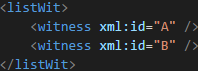
\includegraphics[scale=0.6667]{../graphics/listwit-xml.png}
				
				\vspace{\baselineskip}
				
				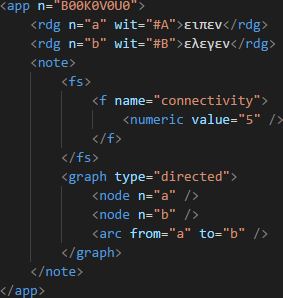
\includegraphics[scale=0.6667]{../graphics/app-xml.png}
			\end{column}
			\begin{column}{0.55\textwidth}
				\begin{itemize}
					\item Database is populated from a collation file in TEI XML format
					\item With a SQLite database, the entire process can be done locally
					\item This makes the distribution itself lightweight and portable
				\end{itemize}
				\begin{table}
					\footnotesize
					\begin{tabular}{l|l|l}
						XML & Object & DB Table\\
						\hline
						\hline
						\texttt{witness} & Witness & \texttt{WITNESSES}\\
						\hline
						\texttt{app} & Variant passage & \texttt{VARIATION\_}\\
						 & & \texttt{UNITS}\\
						 \hline
						\texttt{rdg} & Variant reading & \texttt{READINGS}\\
						\hline
						\texttt{graph} & Local stemma & \texttt{READING\_}\\
						 & & \texttt{RELATIONS}
					\end{tabular}
				\end{table}
			\end{column}
		\end{columns}
	\end{frame}
	\begin{frame}{Local Stemmata}
		\begin{columns}
			\begin{column}{0.4\textwidth}
				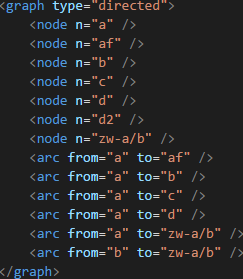
\includegraphics[scale=0.6667]{../graphics/local-stemma-xml.png}
			\end{column}
			\begin{column}{0.55\textwidth}
				\begin{itemize}
					\item Local stemmata are fully customizable in the XML input
				\end{itemize}
				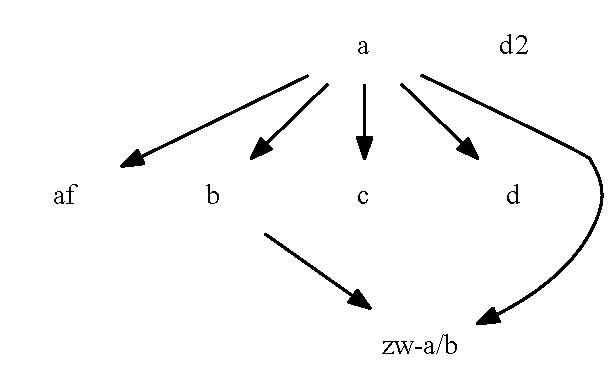
\includegraphics[width=\textwidth]{../graphics/B25K1V4U22-26-local-stemma-no-legend.pdf}
			\end{column}
		\end{columns}
	\end{frame}
	\begin{frame}{Local Stemmata}
		\begin{itemize}
			\item Reading types can be collapsed
		\end{itemize}
		\begin{figure}
			\centering
			\texttt{-z defective -z ambiguous}
			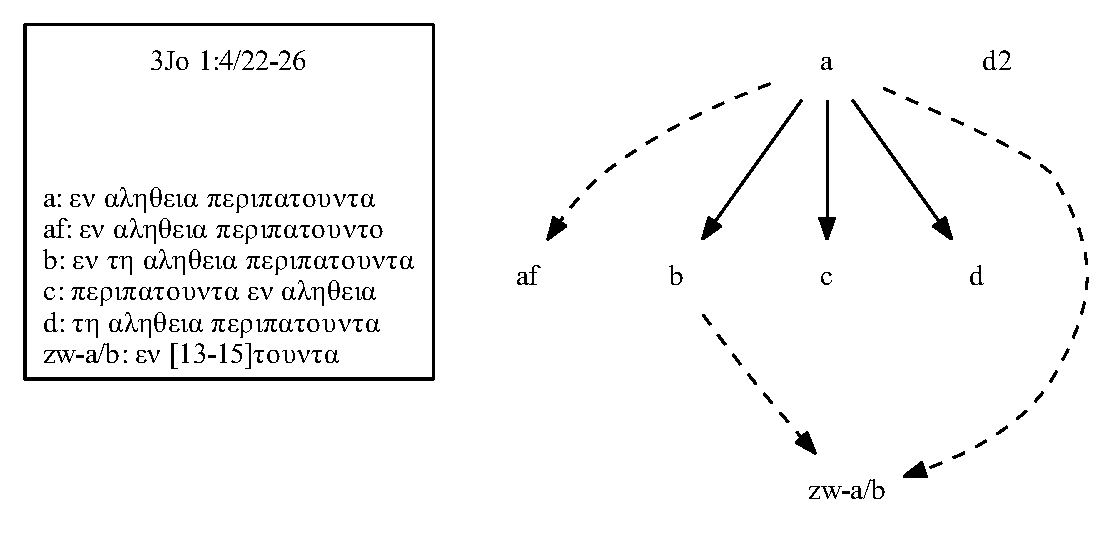
\includegraphics[width=\textwidth]{../graphics/B25K1V4U22-26-local-stemma-ignore-defective-ignore-ambiguous.pdf}
		\end{figure}
	\end{frame}
	\begin{frame}{Local Stemmata}
		\begin{itemize}
			\item Reading types can be dropped
		\end{itemize}
		\begin{figure}
			\centering
			\texttt{-z defective -Z ambiguous}
			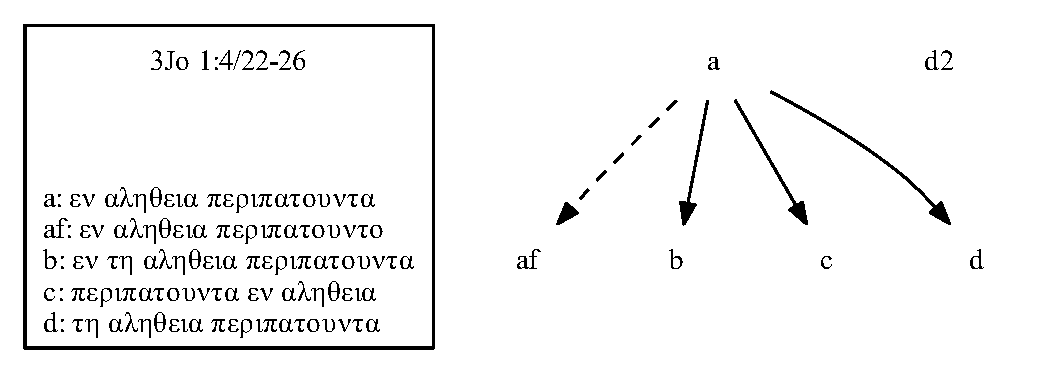
\includegraphics[width=\textwidth]{../graphics/B25K1V4U22-26-local-stemma-ignore-defective-drop-ambiguous.pdf}
		\end{figure}
	\end{frame}
	\begin{frame}{Local Stemmata}
		\begin{itemize}
			\item Split attestations can be merged
		\end{itemize}
		\begin{figure}
			\centering
			\texttt{-z defective -Z ambiguous --merge-splits}
			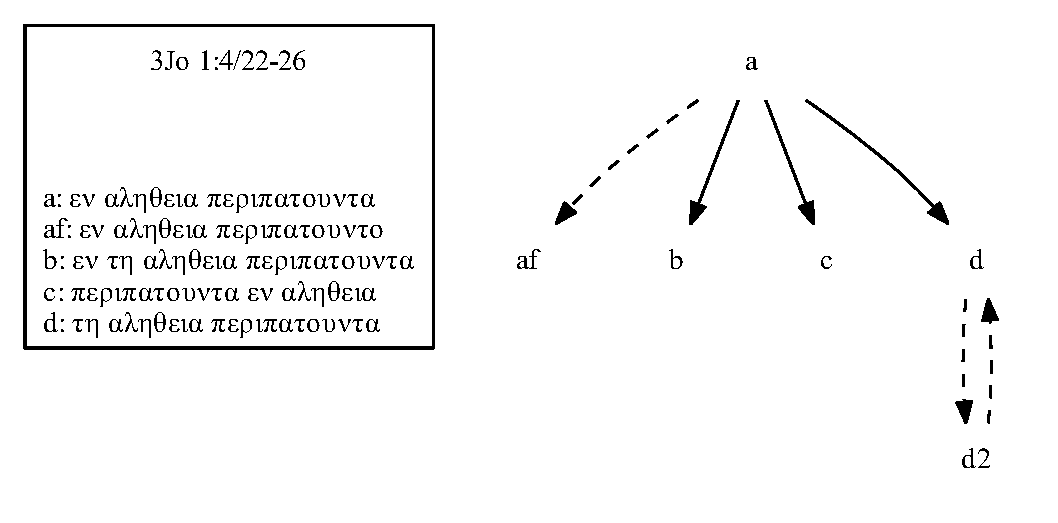
\includegraphics[width=\textwidth]{../graphics/B25K1V4U22-26-local-stemma-ignore-defective-drop-ambiguous-merge-splits.pdf}
		\end{figure}
	\end{frame}
	\begin{frame}{Genealogical Relationships}
		\begin{itemize}
			\item The \texttt{open-cbgm} library encodes genealogical relationships relative to a given witness as bitmaps (one bit per passage)
		\end{itemize}
		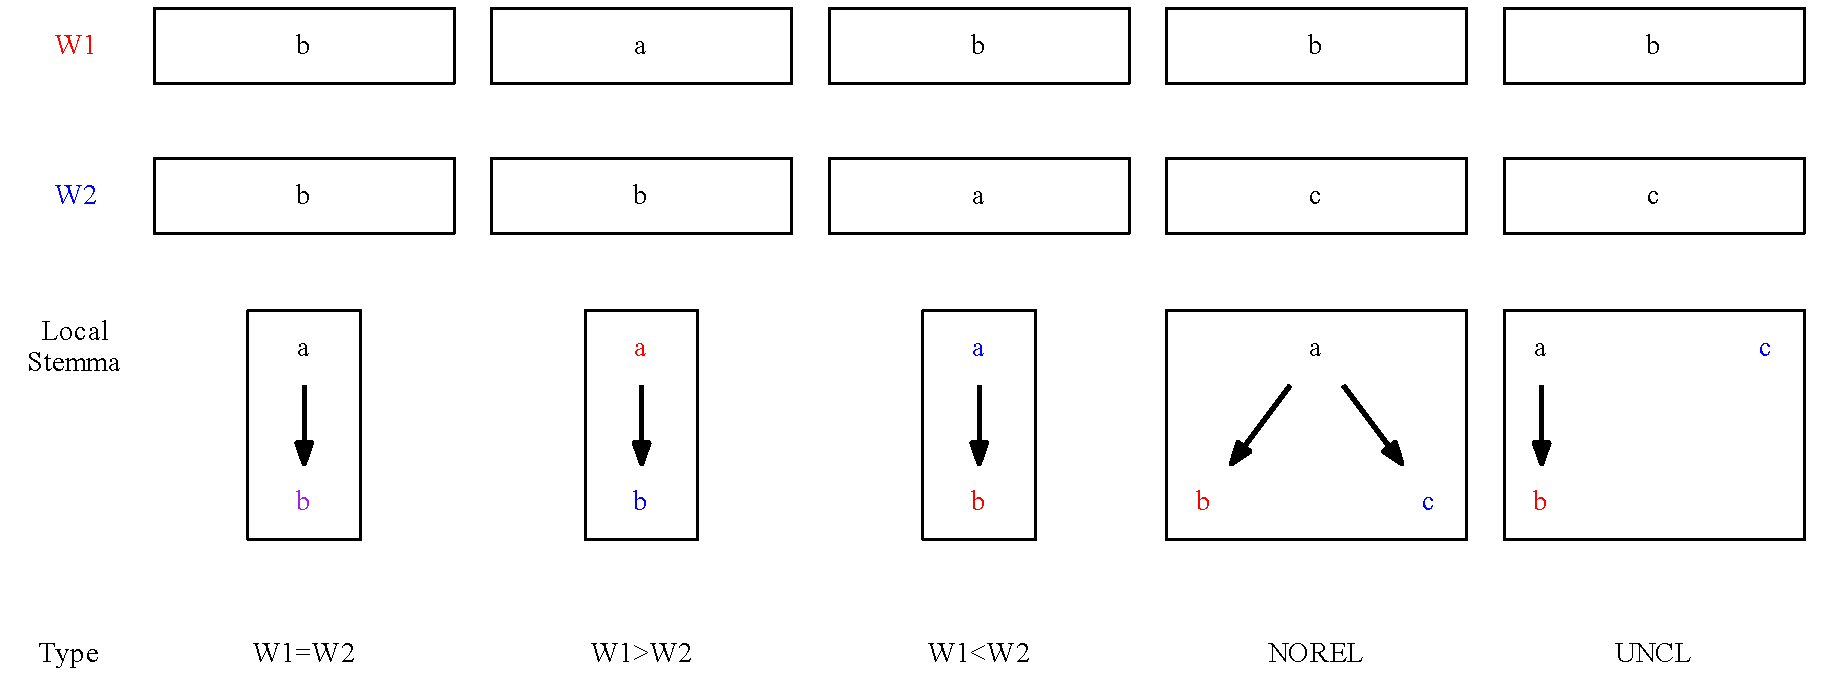
\includegraphics[width=\textwidth]{../graphics/genealogical-relationships.pdf}
		\begin{columns}
			\begin{column}{0.5\textwidth}
				\begin{align*}
					\mathtt{agree} &= [1,0,0,0,0]^{\color{orange}\star}\\
					\mathtt{prior} &= [0,1,0,0,0]\\
					\mathtt{posterior} &= [0,0,1,0,0]
				\end{align*}
			\end{column}
			\begin{column}{0.5\textwidth}
				\begin{align*}
					\mathtt{norel} &= [0,0,0,1,0]\\
					\mathtt{uncl} &= [0,0,0,0,1]\\
					\mathtt{expl} &= [1,0,1,0,0]^{\color{orange}\star}
				\end{align*}
			\end{column}
		\end{columns}
	\end{frame}
	\begin{frame}{Criteria for Explained Readings}
		\begin{columns}
			\begin{column}{0.4\textwidth}
				\centering
				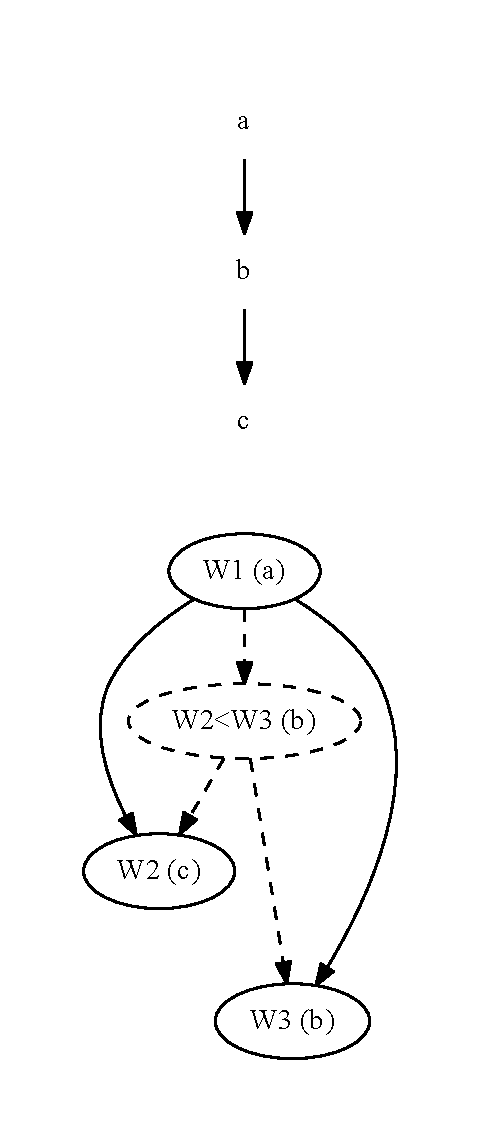
\includegraphics[width=0.75\textwidth]{../graphics/intermediary-node-example.pdf}
			\end{column}
			\begin{column}{0.55\textwidth}
				\begin{itemize}
					\item In the local stemma to the left, does \emph{a} explain \emph{c}?
					\item The ``classic'' rules of the CBGM as implemented by CCeH and Edmondson say \emph{no}: the explaining reading must agree with or be directly prior to the explained reading
					\item Intermediary nodes may be needed to connect the global stemma
				\end{itemize}
			\end{column}
		\end{columns}
	\end{frame}
	\begin{frame}{Criteria for Explained Readings}
		\begin{columns}
			\begin{column}{0.4\textwidth}
				\centering
				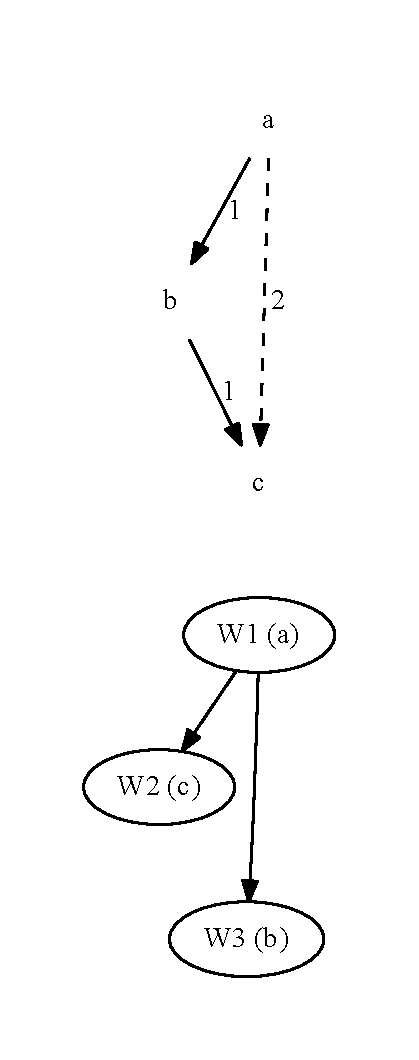
\includegraphics[width=0.75\textwidth]{../graphics/transitivity-example.pdf}
			\end{column}
			\begin{column}{0.55\textwidth}
				\begin{itemize}
					\item The \texttt{open-cbgm} implementation relaxes this criterion: any reading with a path in the local stemma to the reading in question explains it
					\item No intermediary nodes needed (but multiple changes in the same passage may be implied along the edges)
				\end{itemize}
			\end{column}
		\end{columns}
	\end{frame}
%	\begin{frame}{Genealogical Relationship Costs}
%		\begin{columns}
%			\begin{column}{0.4\textwidth}
%				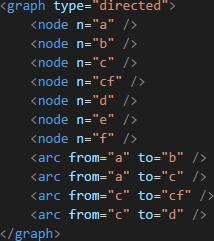
\includegraphics[scale=0.6667]{../graphics/B25K1V13U24-26-local-stemma-xml.png}
%			\end{column}
%			\begin{column}{0.55\textwidth}
%				\begin{itemize}
%					\item In ``classic'' rules, cost = $0$ for agreement, $1$ for disagreement
%					\item ``Agreement'': same reading or readings connected only by dashed edges
%					\item Uniform weight for all passages
%				\end{itemize}
%				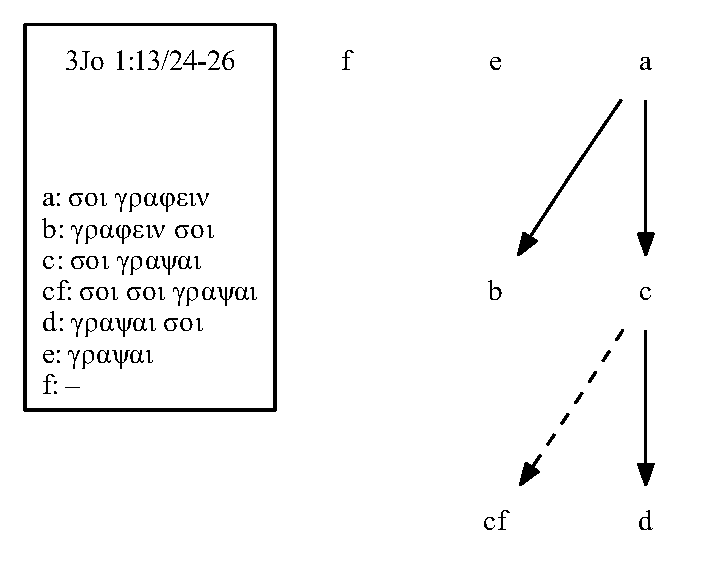
\includegraphics[width=\textwidth]{../graphics/B25K1V13U24-26-local-stemma.pdf}
%			\end{column}
%		\end{columns}
%	\end{frame}
	\begin{frame}{Genealogical Relationship Costs}
		\begin{columns}
			\begin{column}{0.4\textwidth}
				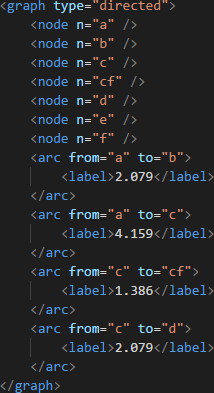
\includegraphics[scale=0.6667]{../graphics/B25K1V13U24-26-local-stemma-weighted-xml.png}
			\end{column}
			\begin{column}{0.55\textwidth}
				\begin{itemize}
					\item In \texttt{open-cbgm}, cost = shortest path length
					\item Edge weights in \texttt{label} element 
					\item Example: scribal change log-likelihood $w = -\log p$
				\end{itemize}
				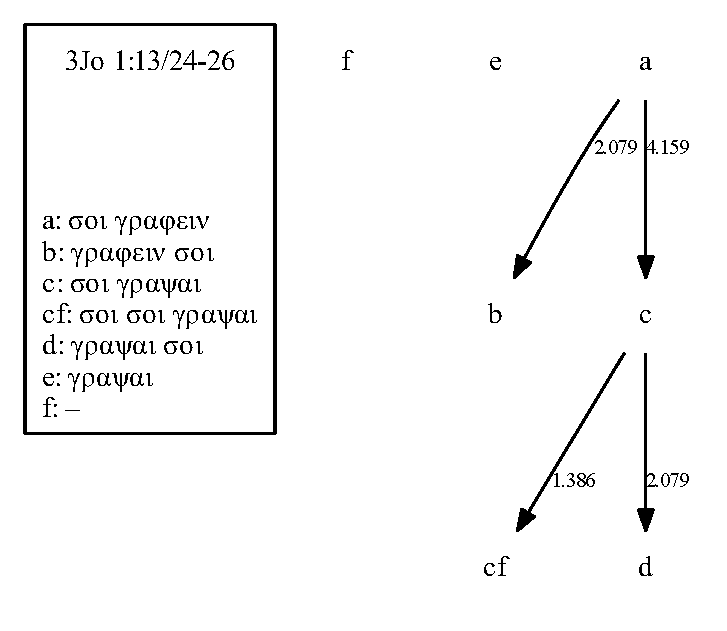
\includegraphics[width=\textwidth]{../graphics/B25K1V13U24-26-local-stemma-weighted.pdf}
			\end{column}
		\end{columns}
	\end{frame}
	\begin{frame}{Substemma Optimization}
		\begin{table}
			\centering
			\begin{tabular}{lrr}
				Ancestor & Explained & Cost\\
				\hline
				A & $[1,1,1,1]$ & $3$\\
				B & $[1,1,0,0]$ & $1$\\
				C & $[0,1,1,1]$ & $1$\\
			\end{tabular}
		\end{table}
		\begin{itemize}
			\item Substemma optimization can be cast as a \emph{weighted set cover} problem
			\item Example: witness D, extant in four passages, has three potential ancestors A, B, and C
			\item The substemma \{A\} is \emph{feasible}, in that it covers all of D's passages (i.e., explains D's readings at all of them)
			\item But \{B, C\} is feasible and \emph{optimal} in terms of total cost ($2$ rather than $3$)
		\end{itemize}
	\end{frame}
	\begin{frame}{Substemma Optimization}
		\begin{columns}
			\begin{column}{0.4\textwidth}
				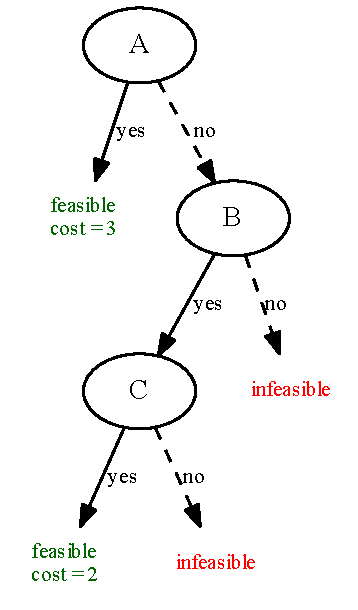
\includegraphics[width=\textwidth]{../graphics/branch-and-bound-example.pdf}
			\end{column}
			\begin{column}{0.55\textwidth}
				\begin{itemize}
					\item For a witness with $n$ potential ancestors, evaluating all of its $2^n$ possible substemmata by brute force would be prohibitive
					\item The \emph{branch-and-bound} heuristic (pictured left) finds all minimum-cost substemmata quickly in practice
					\item Easily adpated to find all substemmata within a given cost
				\end{itemize}
			\end{column}
		\end{columns}
	\end{frame}
	\begin{frame}{CBGM Iterative Workflow}
		\begin{center}
			DEMO
		\end{center}
	\end{frame}
	\begin{frame}{Conclusion}
		\begin{itemize}
			\item The \texttt{open-cbgm} core library is freely available at \url{https://github.com/jjmccollum/open-cbgm}, and the standalone command-line utility is available at \url{https://github.com/jjmccollum/open-cbgm-standalone}
			\item Supported on Windows, Mac, and Linux
			\item A more user-friendly web interface is being co-developed with Tim and Jessie Stoel (Phoenix Seminary)
			\item Currently being used by David Flood (University of Edinburgh) for his PhD dissertation on GA 0150, 1506 and 2110
		\end{itemize}
	\end{frame}
	\begin{frame}[allowframebreaks]
		\printbibliography
	\end{frame}
	\begin{frame}{Appendix: Comparison of CBGM Implementations}
		\begin{table}
			\centering
			\begin{tabular}{p{6em}p{6em}p{6em}p{4em}}
				 & \phantom{text}\newline INTF/CCeH & \phantom{text}\newline Edmondson & \texttt{open-}\newline\texttt{cbgm}\\
				\hline
				\hline
				Input format & MySQL DB & Python script & TEI XML\\
				\hline
				Textual flow ancestry constrained by local stemma edges? & No & Yes & No\\
				\hline
				Lacunose witnesses allowed in textual flow? & Yes (CCeH) & No & Yes
			\end{tabular}
		\end{table}
	\end{frame}
	\begin{frame}{Appendix: Comparison of CBGM Implementations}
		\begin{table}
			\centering
			\begin{tabular}{p{6em}p{6em}p{6em}p{4em}}
				 & \phantom{text}\newline INTF/CCeH & \phantom{text}\newline Edmondson & \texttt{open-}\newline\texttt{cbgm}\\
				\hline
				\hline
				Explanation only by same or parent reading? & Yes & Yes & No\\
				\hline
				Supports weighted input? & No & No & Yes\\
				\hline
				Genealogical cost function & Disagreement & Disagreement & Shortest path length\\
				\hline
				Intermediary nodes needed? & Yes & Yes & No
			\end{tabular}
		\end{table}
	\end{frame}
\end{document}